\subsection{Paquete 1: Gestión de identidad, sesión y perfil}

    El paquete centraliza el registro de cuentas, la expedición y rotación de tókenes de seguridad, el restablecimiento de contraseñas y el ciclo de vida del perfil. La figura \ref{fig:dcu_identidad} representa las relaciones entre los actores y los quince casos de uso del módulo.

\begin{figure}[H]
    \centering
    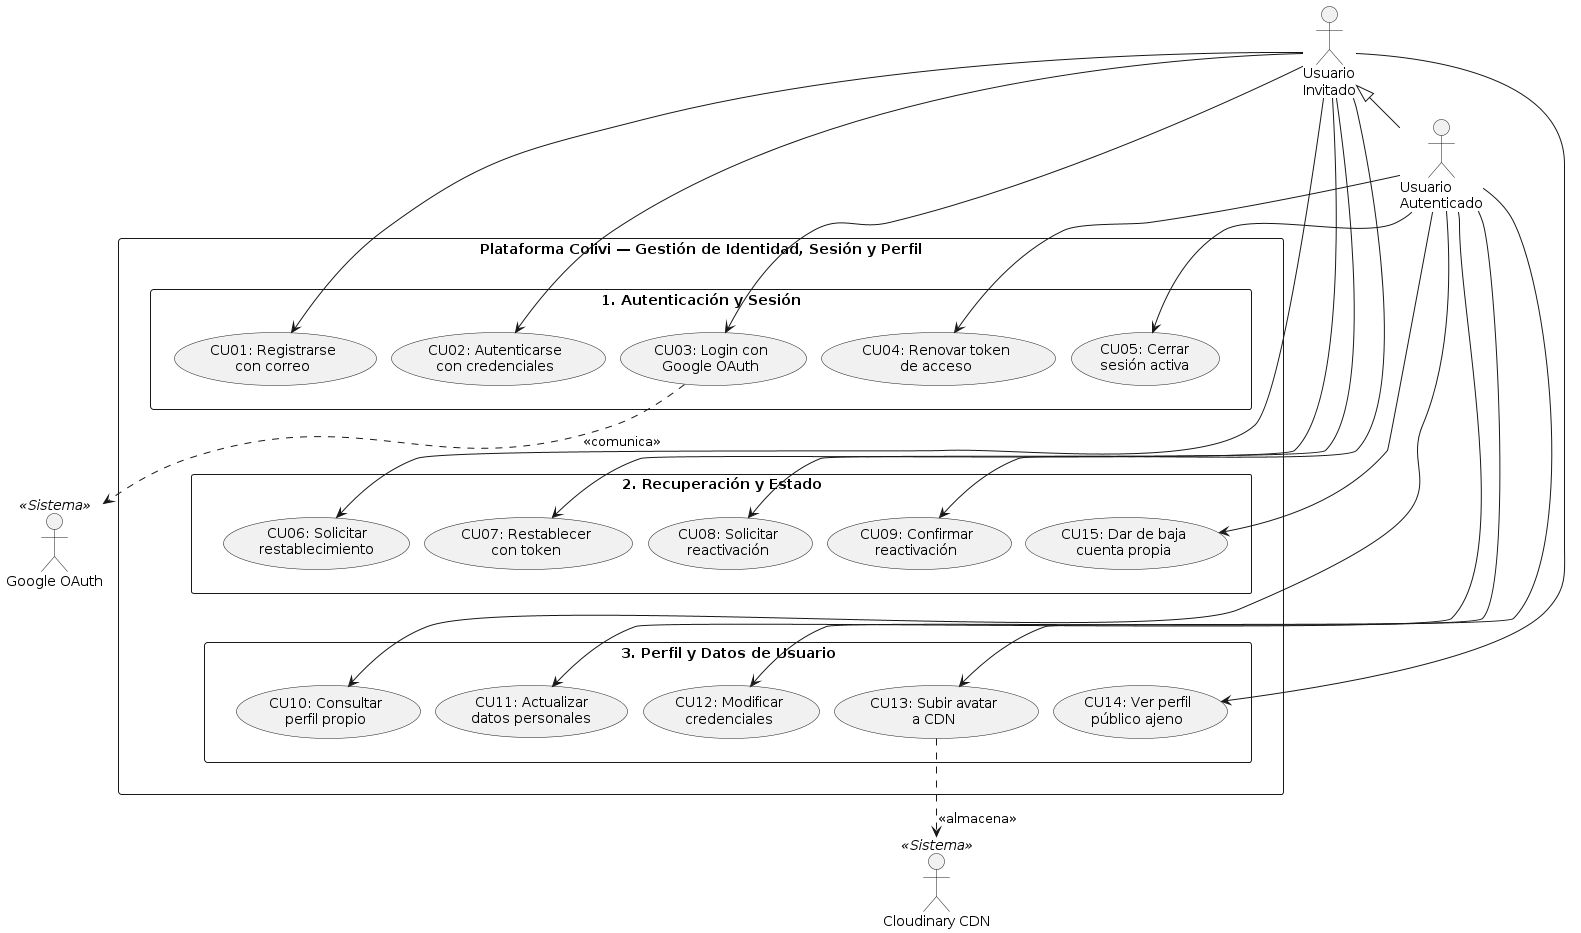
\includegraphics[width=0.95\textwidth]{AnalisisFuncional/img/dcu_identidad.png}
    \caption{Diagrama de casos de uso del módulo de identidad, sesión y perfil}
    \label{fig:dcu_identidad}
\end{figure}

    Las siguientes tablas recogen la especificación formal de cada caso de uso:

\begin{table}[H]
\centering
\begin{tabular}{|p{3.1cm}|p{10.9cm}|}
\hline
\textbf{Caso de Uso} & \textbf{CU01: Registrarse con correo y contraseña} \\ \hline
\textbf{Actores} & Usuario Invitado \\ \hline
\textbf{Descripción} & Permite a un nuevo usuario crear una cuenta local mediante credenciales \\ \hline
\textbf{Precondiciones} & No poseer una sesión activa y que el correo no figure previamente registrado \\ \hline
\textbf{Flujo básico} & 
1. El usuario accede al formulario de registro en la interfaz de usuario. \newline
2. El usuario introduce nombre, apellidos, dirección de correo electrónico y contraseña. \newline
3. El sistema valida el formato de los datos y comprueba la disponibilidad del correo. \newline
4. El sistema almacena la credencial protegida con un algoritmo de dispersión criptográfica y confirma la creación de la cuenta. \\ \hline
\end{tabular}
\caption{Especificación del caso de uso CU01.}
\label{tab:cu01}
\end{table}

\begin{table}[H]
\centering
\begin{tabular}{|p{3.1cm}|p{10.9cm}|}
\hline
\textbf{Caso de Uso} & \textbf{CU02: Autenticarse con credenciales} \\ \hline
\textbf{Actores} & Usuario Invitado \\ \hline
\textbf{Descripción} & Valida las credenciales locales para expedir una sesión sin estado \\ \hline
\textbf{Precondiciones} & Estar registrado y que la cuenta no se encuentre dada de baja o suspendida \\ \hline
\textbf{Flujo básico} & 
1. El usuario accede a la vista de inicio de sesión e introduce correo y contraseña. \newline
2. El sistema valida la coincidencia de las credenciales frente a la base de datos. \newline
3. El sistema genera un par de tókenes JWT (acceso y renovación) con los roles asignados. \newline
4. El cliente almacena los tókenes de manera segura y redirige al panel principal. \\ \hline
\end{tabular}
\caption{Especificación del caso de uso CU02.}
\label{tab:cu02}
\end{table}

\begin{table}[H]
\centering
\begin{tabular}{|p{3.1cm}|p{10.9cm}|}
\hline
\textbf{Caso de Uso} & \textbf{CU03: Autenticarse mediante Google OAuth} \\ \hline
\textbf{Actores} & Usuario Invitado, Google OAuth \\ \hline
\textbf{Descripción} & Permite iniciar sesión o registrarse mediante delegación de identidad federada \\ \hline
\textbf{Precondiciones} & Poseer una cuenta activa y verificada en el proveedor Google \\ \hline
\textbf{Flujo básico} & 
1. El usuario pulsa sobre la opción de acceso con Google en la interfaz. \newline
2. El proveedor solicita el consentimiento y devuelve un token de identidad criptográfico. \newline
3. El backend verifica la autenticidad del token frente a los servidores de Google. \newline
4. El sistema localiza la cuenta existente o crea un nuevo registro sincronizado, emitiendo la sesión JWT local. \\ \hline
\end{tabular}
\caption{Especificación del caso de uso CU03.}
\label{tab:cu03}
\end{table}

\begin{table}[H]
\centering
\begin{tabular}{|p{3.1cm}|p{10.9cm}|}
\hline
\textbf{Caso de Uso} & \textbf{CU04: Renovar token de acceso} \\ \hline
\textbf{Actores} & Usuario Autenticado \\ \hline
\textbf{Descripción} & Obtiene un nuevo token de acceso antes o tras la expiración del vigente \\ \hline
\textbf{Precondiciones} & Disponer de un token de renovación válido y no revocado \\ \hline
\textbf{Flujo básico} & 
1. El cliente detecta la caducidad del token de acceso durante una petición a la API. \newline
2. El cliente envía el token de renovación a la ruta de refresco del servidor. \newline
3. El backend comprueba la integridad del token y la vigencia del usuario. \newline
4. El sistema expide y devuelve un nuevo token de acceso de corta duración. \\ \hline
\end{tabular}
\caption{Especificación del caso de uso CU04.}
\label{tab:cu04}
\end{table}

\begin{table}[H]
\centering
\begin{tabular}{|p{3.1cm}|p{10.9cm}|}
\hline
\textbf{Caso de Uso} & \textbf{CU05: Cerrar sesión activa} \\ \hline
\textbf{Actores} & Usuario Autenticado \\ \hline
\textbf{Descripción} & Finaliza la sesión actual y purga las credenciales del cliente \\ \hline
\textbf{Precondiciones} & Mantener una sesión activa en la aplicación \\ \hline
\textbf{Flujo básico} & 
1. El usuario pulsa la acción de cierre de sesión en el menú de navegación. \newline
2. El cliente elimina los tókenes de acceso y renovación almacenados localmente. \newline
3. El sistema invalida la caché de consultas asíncronas y redirige a la vista de inicio. \\ \hline
\end{tabular}
\caption{Especificación del caso de uso CU05.}
\label{tab:cu05}
\end{table}

\begin{table}[H]
\centering
\begin{tabular}{|p{3.1cm}|p{10.9cm}|}
\hline
\textbf{Caso de Uso} & \textbf{CU06: Solicitar restablecimiento de contraseña} \\ \hline
\textbf{Actores} & Usuario Invitado \\ \hline
\textbf{Descripción} & Inicia el protocolo de recuperación de acceso mediante correo electrónico \\ \hline
\textbf{Precondiciones} & Que la cuenta asociada al correo exista en la plataforma \\ \hline
\textbf{Flujo básico} & 
1. El usuario introduce su dirección de correo en la vista de contraseña olvidada. \newline
2. El sistema comprueba la existencia del registro sin desvelar información sensible. \newline
3. El sistema genera un token de un solo uso con caducidad temporal de quince minutos. \newline
4. El servicio de correo despacha un mensaje con el enlace firmado para el restablecimiento. \\ \hline
\end{tabular}
\caption{Especificación del caso de uso CU06.}
\label{tab:cu06}
\end{table}

\begin{table}[H]
\centering
\begin{tabular}{|p{3.1cm}|p{10.9cm}|}
\hline
\textbf{Caso de Uso} & \textbf{CU07: Restablecer contraseña con token seguro} \\ \hline
\textbf{Actores} & Usuario Invitado \\ \hline
\textbf{Descripción} & Actualiza la contraseña de la cuenta consumiendo el enlace de recuperación \\ \hline
\textbf{Precondiciones} & Acceder con un token de restablecimiento vigente y no consumido \\ \hline
\textbf{Flujo básico} & 
1. El usuario abre el enlace recibido e introduce una nueva contraseña. \newline
2. El sistema valida las políticas de complejidad de la nueva clave. \newline
3. El backend verifica la validez temporal del token y actualiza la credencial cifrada. \newline
4. El sistema revoca el token utilizado y redirige a la vista de inicio de sesión. \\ \hline
\end{tabular}
\caption{Especificación del caso de uso CU07.}
\label{tab:cu07}
\end{table}

\begin{table}[H]
\centering
\begin{tabular}{|p{3.1cm}|p{10.9cm}|}
\hline
\textbf{Caso de Uso} & \textbf{CU08: Solicitar reactivación de cuenta} \\ \hline
\textbf{Actores} & Usuario Invitado \\ \hline
\textbf{Descripción} & Permite a un usuario con la cuenta desactivada voluntariamente solicitar el enlace de reactivación \\ \hline
\textbf{Precondiciones} & Disponer de una cuenta registrada previamente en estado desactivado \\ \hline
\textbf{Flujo básico} & 
1. El usuario introduce su dirección de correo electrónico en el formulario de reactivación. \newline
2. El sistema comprueba que la cuenta existe y se encuentra en estado inactivo. \newline
3. El sistema genera un token criptográfico de reactivación con validez temporal. \newline
4. El servicio de correo despacha un mensaje con el enlace firmado para confirmar el restablecimiento de la cuenta. \\ \hline
\end{tabular}
\caption{Especificación del caso de uso CU08.}
\label{tab:cu08}
\end{table}

\begin{table}[H]
\centering
\begin{tabular}{|p{3.1cm}|p{10.9cm}|}
\hline
\textbf{Caso de Uso} & \textbf{CU09: Confirmar reactivación de cuenta} \\ \hline
\textbf{Actores} & Usuario Invitado \\ \hline
\textbf{Descripción} & Restablece el estado activo de la cuenta consumiendo el enlace de verificación recibido \\ \hline
\textbf{Precondiciones} & Acceder mediante un token de reactivación válido y no expirado \\ \hline
\textbf{Flujo básico} & 
1. El usuario accede a la plataforma a través del enlace de reactivación. \newline
2. El backend valida la firma criptográfica y la vigencia temporal del token. \newline
3. El sistema actualiza el estado de la cuenta a activo en la base de datos. \newline
4. El sistema redirige al usuario al formulario de autenticación notificando el éxito del proceso. \\ \hline
\end{tabular}
\caption{Especificación del caso de uso CU09.}
\label{tab:cu09}
\end{table}

\begin{table}[H]
\centering
\begin{tabular}{|p{3.1cm}|p{10.9cm}|}
\hline
\textbf{Caso de Uso} & \textbf{CU10: Consultar perfil propio} \\ \hline
\textbf{Actores} & Usuario Autenticado \\ \hline
\textbf{Descripción} & Muestra la información personal, preferencias de convivencia, valoraciones y estado de verificación del usuario actual \\ \hline
\textbf{Precondiciones} & Mantener una sesión activa en la aplicación \\ \hline
\textbf{Flujo básico} & 
1. El usuario accede a la sección de perfil desde la barra de navegación. \newline
2. El sistema recupera los datos del usuario, métricas de actividad y configuración asociada. \newline
3. La interfaz renderiza la información personal organizada en secciones editables. \\ \hline
\end{tabular}
\caption{Especificación del caso de uso CU10.}
\label{tab:cu10}
\end{table}

\begin{table}[H]
\centering
\begin{tabular}{|p{3.1cm}|p{10.9cm}|}
\hline
\textbf{Caso de Uso} & \textbf{CU11: Actualizar datos personales} \\ \hline
\textbf{Actores} & Usuario Autenticado \\ \hline
\textbf{Descripción} & Permite modificar el nombre, teléfono, biografía académica o profesional y preferencias de convivencia \\ \hline
\textbf{Precondiciones} & Sesión activa y datos introducidos conformes a las restricciones de validación \\ \hline
\textbf{Flujo básico} & 
1. El usuario edita los campos deseados en el formulario de perfil. \newline
2. El cliente valida el formato de los datos introducidos. \newline
3. El backend persiste las modificaciones en la base de datos. \newline
4. La interfaz actualiza la vista reflejando los nuevos datos confirmados. \\ \hline
\end{tabular}
\caption{Especificación del caso de uso CU11.}
\label{tab:cu11}
\end{table}

\begin{table}[H]
\centering
\begin{tabular}{|p{3.1cm}|p{10.9cm}|}
\hline
\textbf{Caso de Uso} & \textbf{CU12: Modificar credenciales} \\ \hline
\textbf{Actores} & Usuario Autenticado \\ \hline
\textbf{Descripción} & Permite sustituir la contraseña de acceso actual por una nueva clave segura \\ \hline
\textbf{Precondiciones} & Estar autenticado con credenciales locales y conocer la contraseña vigente \\ \hline
\textbf{Flujo básico} & 
1. El usuario introduce la contraseña actual y la nueva clave junto con su confirmación. \newline
2. El sistema verifica que la contraseña actual coincida con el resumen criptográfico almacenado. \newline
3. El sistema comprueba las directivas de seguridad y complejidad de la nueva clave. \newline
4. El backend genera el nuevo hash criptográfico, actualiza el registro y revoca las sesiones previas. \\ \hline
\end{tabular}
\caption{Especificación del caso de uso CU12.}
\label{tab:cu12}
\end{table}

\begin{table}[H]
\centering
\begin{tabular}{|p{3.1cm}|p{10.9cm}|}
\hline
\textbf{Caso de Uso} & \textbf{CU13: Subir avatar a CDN} \\ \hline
\textbf{Actores} & Usuario Autenticado, Cloudinary CDN \\ \hline
\textbf{Descripción} & Permite cargar o sustituir la fotografía de perfil del usuario mediante almacenamiento en la nube \\ \hline
\textbf{Precondiciones} & Archivo gráfico en formato admitido inferior al límite de tamaño permitido \\ \hline
\textbf{Flujo básico} & 
1. El usuario selecciona una imagen desde el almacenamiento local de su dispositivo. \newline
2. El cliente transfiere de forma segura el archivo multimedia al servicio Cloudinary. \newline
3. El CDN procesa, optimiza y almacena la imagen, retornando su identificador y enlace seguro HTTPS. \newline
4. El backend asocia la nueva URL al perfil del usuario y elimina el recurso anterior si procede. \\ \hline
\end{tabular}
\caption{Especificación del caso de uso CU13.}
\label{tab:cu13}
\end{table}

\begin{table}[H]
\centering
\begin{tabular}{|p{3.1cm}|p{10.9cm}|}
\hline
\textbf{Caso de Uso} & \textbf{CU14: Ver perfil público ajeno} \\ \hline
\textbf{Actores} & Usuario Autenticado \\ \hline
\textbf{Descripción} & Permite inspeccionar la ficha pública de un potencial compañero de piso o anfitrión, omitiendo información de contacto privada \\ \hline
\textbf{Precondiciones} & Que el perfil consultado exista y pertenezca a un usuario con cuenta activa \\ \hline
\textbf{Flujo básico} & 
1. El usuario pulsa sobre el avatar o nombre de un usuario en un anuncio, mensaje o reseña. \newline
2. El backend filtra los campos sensibles y extrae únicamente la información de visibilidad pública. \newline
3. La interfaz muestra la biografía, estilo de vida, valoraciones recibidas y estado de verificación. \\ \hline
\end{tabular}
\caption{Especificación del caso de uso CU14.}
\label{tab:cu14}
\end{table}

\begin{table}[H]
\centering
\begin{tabular}{|p{3.1cm}|p{10.9cm}|}
\hline
\textbf{Caso de Uso} & \textbf{CU15: Dar de baja cuenta propia} \\ \hline
\textbf{Actores} & Usuario Autenticado \\ \hline
\textbf{Descripción} & Permite al usuario solicitar la desactivación o supresión de su cuenta y sus datos personales de la plataforma \\ \hline
\textbf{Precondiciones} & No mantener contratos de alquiler vigentes, deudas pendientes ni reservas activas \\ \hline
\textbf{Flujo básico} & 
1. El usuario selecciona la opción de baja en los ajustes de seguridad e introduce su contraseña de confirmación. \newline
2. El sistema audita la ausencia de bloqueos operativos, tales como estancias en curso o deudas en convivencias activas. \newline
3. El backend marca la cuenta como inactiva o anonimiza los datos según la política de privacidad. \newline
4. El sistema cierra la sesión activa, revoca los tókenes emitidos y redirige a la vista inicial. \\ \hline
\end{tabular}
\caption{Especificación del caso de uso CU15.}
\label{tab:cu15}
\end{table}